\chapter{Problem description}
\begin{figure}[h]
	\centering
	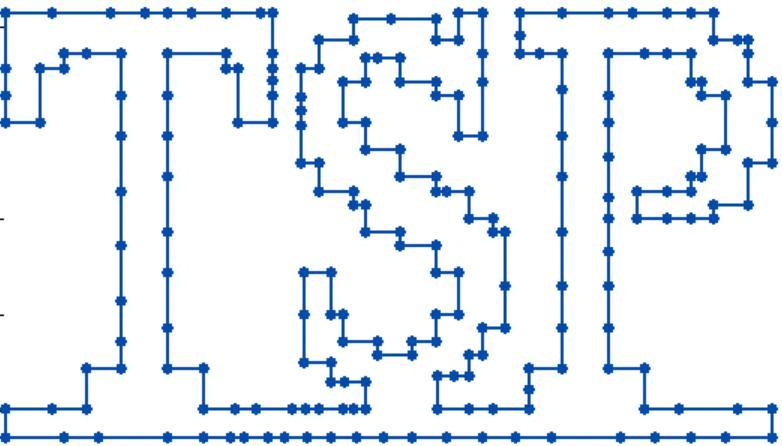
\includegraphics[width=.5\columnwidth]{img/tsp225_plot}
	\caption{The \textit{tsp225.tsp} instance from \textit{tsplib} resolved with \textit{subtour} method described in cap \ref{sec:subtour} plotted by Gnuplot.}
	\label{fig:tsp225}
\end{figure}

The Traveling Salesman Problem is a well-known NP-hard problem. In short, given a set of cities it's required to find the shortest tour that visit exactly one time each city and return to the first one.
In this report two version of the TSP will be analyzed in details:
\begin{itemize}
	\item symmetric TSP (STSP): with bidirectional edges;
 	\item asymmetric TSP (ATSP): with oriented arches.
\end{itemize}


\section{Symmetric TSP}
Given a complete graph $ G = (V, E) $, a distance function $ d $ where:
\begin{itemize}
	\item $ V := \{1, 2, .., n\}$ is a set of nodes;
	\item $ E $ is the set of edges between each node pairs $ i,j \in V, i \ne j $ represented with $ (i,j) $ or for a generic edge $ e $, note that for STSP $ (i,j) = (j,i) $ therefore the number of edges $ |E| = \frac{n(n-1)}{2} $;
	\item $ d: (i,j) = e \to d(i,j) = c_e $ where $ c_e $ is the cost associated to $ e \in E $;
\end{itemize}
and defining the decision variable:
\[
x_e := \begin{cases}
	1 & \text{if $ e $ is in the tour,} \\
	0 & \text{otherwise}
\end{cases}
\] 
the STSP can be represented with linear programming system in \ref{eq:STSP_LP}. 
\begin{equation}
\begin{cases}
		min \sum_{ e\in E } c_ex_e & \text{Cost function} \\
		\sum_{e\in \delta (v) } x_e = 2, \forall v \in V  & \text{Degree constraint} \\
		\sum_{e\in E(S) } x_e \le |S|-1, \forall S \subset V, |S| \ge 3  & \text{Subtour elimination} \\
		x_e \in \{0,1\}, \forall e \in E & \text{Domain constraint}
\end{cases}
\label{eq:STSP_LP}
\end{equation} 
As usual it is required to find the value of $ x_e, \forall e \in E $ that minimize the \textit{cost function} and verify the constraints.
For the \textit{degree constrain}, the degree of each $ v \in V $ ($ |\delta(v)| $) must be equal to 2. A system with only the degree constrain (and the domain constraint) would probably have a set of subtour with size three or more, however adding the \textit{subtour elimination} constraints  it's impose to have only one tour. 

The number of possible subset $ S \subset V $ is exponential ($ 2^{n} - \binom{n}{3} -\binom{n}{2} -\binom{n}{1} - 1 $), therefore even a graph with 100 nodes has huge matrix dimension. Note that $ E(S) := \{ e = (i,j): i,j \in S \subset V \}$.
Considering the example in figure \ref{fig:symTSP}, the value of the solution is represented in the matrix in figure \ref{tab:symTSP_solution} where $ x_{ij} = x_{ji} $ for each $ i,j \in V, i \ne j $ but only the cell with $ i < j $ have been completed to enhance the number of variable that are used in practice.
\begin{figure}[h]
	\centering
	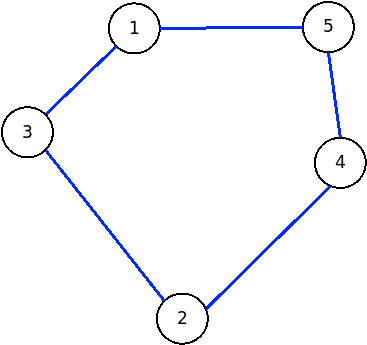
\includegraphics[width=.2\columnwidth]{img/symTSP_example.png}
	\caption{Example of tour. Only the selected edges are visible.}
	\label{fig:symTSP}
\end{figure}

\begin{table}[h!]
	\begin{center}
		\caption{Decision variable matrix. It show the value $ x_{ij} $ of the solution represented in figure \ref{fig:symTSP}. Due to the symmetry of the matrix, only the cell with $ i < j $ have a value, the others can be checked from the first.}
		\label{tab:symTSP_solution}
		\begin{tabular}{cc|c|c|c|c|c|}
			 \multicolumn{2}{c}{} & \multicolumn{5}{c}{j} \\ % <-- Combining two cells with alignment c| and content 12.
			& \multicolumn{1}{c}{} & \multicolumn{1}{c}{1} & \multicolumn{1}{c}{2} & \multicolumn{1}{c}{3} & \multicolumn{1}{c}{4} & \multicolumn{1}{c}{5} \\ \cline{3-7}
			\multirow{5}{*}{i} 	& 1 & \cellcolor{Black} & 0 & 1 & 0 & 1 \\ \cline{3-7}
								& 2 &  & \cellcolor{Black} & 1 & 1 & 0 \\ \cline{3-7}
								& 3 &  &  & \cellcolor{Black} & 0 & 0 \\ \cline{3-7}
								& 4 &  &  &  & \cellcolor{Black} & 1 \\ \cline{3-7}
								& 5 &  &  &  &  & \cellcolor{Black} \\ \cline{3-7}
		\end{tabular}
	\end{center}
\end{table}



\section{Asymmetric TSP}
Given a complete graph $ G = (V,A) $, a distance funciton  $ d $ where:
\begin{itemize}
	\item $ V:= \{1, 2, .., n\} $ is the set of nodes;
	\item $ A := $ the set arches between each nodes $ i,j \in V, i \ne j$ represented as $ (i,j) $, note that in the ATSP $ (i,j) \ne (j,i) $ 
	\item $ d: (i,j) \rightarrow d(i,j) = c_{ij} $ where $ c_{ij} $ is the cost associated to the arch $ (i,j) $
\end{itemize}
and defining the decision variable:
\[
x_{ij} := \begin{cases}
1 & \text{if $ (i,j) $ is in the tour,} \\
0 & \text{otherwise}
\end{cases}
\]
the ATSP can be defined in different ways, in this report two version will be considered: Miller Tucker Zemlin and Flow Chart (by GG).
Note that for the ATSP the number of arches is $ |A| = n*(n-1) $ which is double of the STSP.

\subsection{Miller Tucker Zemlin}
Disegno per la spiegazione dell'origine dei vincoli


\begin{figure}[h]
	\centering
	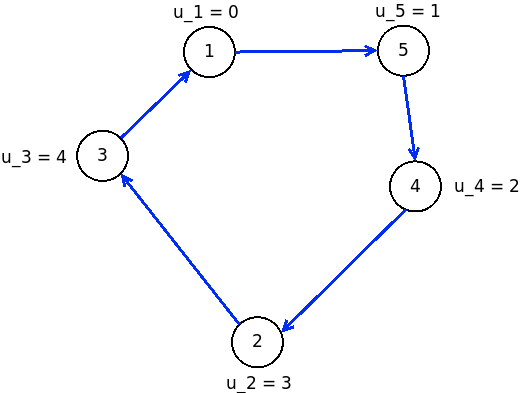
\includegraphics[width=.3\columnwidth]{img/asymTSP_MTZ_example.png}
	\caption{Example of tour. Only the selected arches are visible.}
	\label{fig:asymTSP_MTZ}
\end{figure}

\begin{table}[h!]
	\begin{center}
		\caption{Decision variable matrix. It show the value $ x_{ij}, u_k $ of the solution represented in figure \ref{fig:asymTSP_MTZ}. }
		\label{tab:asymTSP_MTZ_solution}
		\begin{tabular}{cc|c|c|c|c|c|}
			\multicolumn{2}{c}{} & \multicolumn{5}{c}{j} \\ % <-- Combining two cells with alignment c| and content 12.
			& \multicolumn{1}{c}{} & \multicolumn{1}{c}{1} & \multicolumn{1}{c}{2} & \multicolumn{1}{c}{3} & \multicolumn{1}{c}{4} & \multicolumn{1}{c}{5} \\ \cline{3-7}
			\multirow{5}{*}{i} 	& 1 & \cellcolor{Black} & 0 & 0 & 0 & 1 \\ \cline{3-7}
			& 2 & 0 & \cellcolor{Black} & 1 & 0 & 0 \\ \cline{3-7}
			& 3 & 1 & 0 & \cellcolor{Black} & 0 & 0 \\ \cline{3-7}
			& 4 & 0 & 1 & 0 & \cellcolor{Black} & 0 \\ \cline{3-7}
			& 5 & 0 & 0 & 0 & 1 & \cellcolor{Black} \\ \cline{3-7}
			\multicolumn{7}{c}{} \\ 
			
			\multicolumn{2}{c}{} & \multicolumn{5}{c}{$ k $} \\  \cline{3-7}
 			$ u_k $ &  & 0 & 3 & 4 & 2 & 1 \\ \cline{3-7}
		\end{tabular}
	\end{center}
\end{table}

valutazione del numero di vincoli 

\begin{equation}
\begin{cases}
 min \sum_{i\in V}\sum_{j\in V} c_{ij}x_{ij} & \text{Cost function} \\
 \sum_{i\in V} x_{ih} = 1, \forall h \in V  & \text{$ x $ Outer arches} \\
 \sum_{i\in V} x_{hi} = 1, \forall h \in V  & \text{$ x $ Inner arches} \\
u_i -u_j +M x_{ij} \le M - 1, \forall i,j \in V \backslash \{1\} & \text{MTZ constraints} \\
0 \le x_{ij} \le 1, Integer, \forall i,j \in N  & \text{$ x $ Domain} \\
0 \le x_{ii} \le 0, Integer, \forall i \in N  & \text{} \\
0 \le u_{i} \le n-2, Integer, \forall i \in N \backslash \{1\} & \text{$ u $ Domain} 
\end{cases}
\end{equation}

\subsection{Flow Chart}
Disegno per la spiegazione dell'origine dei vincoli


\begin{figure}[h]
	\centering
	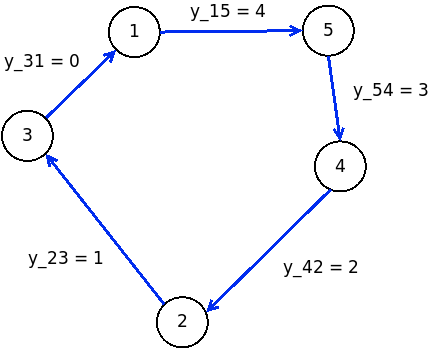
\includegraphics[width=.2\columnwidth]{img/asymTSP_FC_example.png}
	\caption{Example of tour. Only the selected arches are visible.}
	\label{fig:asymTSP_FC}
\end{figure}

\begin{table}[h!]
	\begin{center}
		\caption{Decision variable matrix. It show the value $ x_{ij}, u_k $ of the solution represented in figure \ref{fig:asymTSP}. }
		\label{tab:asymTSP_FC_solution}
		\begin{tabular}{cc|c|c|c|c|c|}
			\multicolumn{2}{c}{} & \multicolumn{5}{c}{j} \\ % <-- Combining two cells with alignment c| and content 12.
			& \multicolumn{1}{c}{} & \multicolumn{1}{c}{1} & \multicolumn{1}{c}{2} & \multicolumn{1}{c}{3} & \multicolumn{1}{c}{4} & \multicolumn{1}{c}{5} \\ \cline{3-7}
			\multirow{5}{*}{i} 	& 1 & \cellcolor{Black} & 0 & 0 & 0 & 1 \\ \cline{3-7}
			& 2 & 0 & \cellcolor{Black} & 1 & 0 & 0 \\ \cline{3-7}
			& 3 & 1 & 0 & \cellcolor{Black} & 0 & 0 \\ \cline{3-7}
			& 4 & 0 & 1 & 0 & \cellcolor{Black} & 0 \\ \cline{3-7}
			& 5 & 0 & 0 & 0 & 1 & \cellcolor{Black} \\ \cline{3-7}
		\end{tabular}
	\end{center}
\end{table}

valutazione del numero di vincoli 
\begin{equation}
\begin{cases}
	min \sum_{i\in V}\sum_{j\in V} c_{ij}x_{ij}  & \text{Cost function} \\
	\sum_{i\in V} x_{ih} = 1, \forall h \in V  & \text{$ x $ Outer arches} \\
	\sum_{i\in V} x_{hi} = 1, \forall h \in V  & \text{$ x $ Inner arches} \\
	\sum_{j\in V} y_{1j} = n-1  & \text{$ 1 $ Outer flow} \\
	\sum_{j\in V} y_{hj} = \sum_{i \in V}y_{ih} - 1, \forall h \in V \backslash \{1\}  & \text{Decreasing flow} \\
	y_{ij} - x_{ij}(n-1) \le 0, \forall i \in V, \forall j \in V \backslash \{1\}  & \text{Cuttling constraints} \\
	0 \le x_{ij} \le 1, Integer, \forall i,j \in N  & \text{$ x $ Domain} \\
	0 \le x_{ii} \le 0, Integer, \forall i \in N & \text{} \\
	0 \le y_{i1} \le 0, \forall i \in V  & \text{$ y $ Domain} \\
	0 \le y_{ii} \le 0, \forall i \in V  & \text{} \\
	0 \le y_{ij} \le n-1, Integer, \forall i,j \in V  & \text{} 
\end{cases}
\end{equation}